\chapter{計算手法}
本章では,Moment法による計算手法,また,比較対象である,Phonon-DOS法,Phonopyについて記述する.

\section{熱膨張決定のアルゴリズム}
\ref{sec:heatexpantion}節で熱膨張による変位の求め方について述べ,$y$=$y_0$の時の$y$が熱膨張による変位だとわかった.
$y_0$は$k$と$\gamma$を介して$y$に依存する関数であり,$y$の変化に合わせて$y_0$を変化することになる.
$y$=$y_0$となる$y$を決定するアルゴリズムは次のようになる.
\begin{enumerate}
 \item 平衡原子間距離$a_0$を定める.
 \item 計算者が決定する変位$y$に一定の値を足す.
 \item $a_0$+$y$から原子間距離が求まる.
 \item 3.の値から$k$, $\gamma$を求める.
 \item $k$, $\gamma$から$y_0$を求める.
 \item $y$が$y_0$を超えるまで2-5.を繰り返す.
 \item $y$が$y_0$を越えたら,越える前まで戻す.
 \item $y$に足していた一定の値を10で割り2.に戻る.
 \item 2-8.を繰り返すことにより,$y=y_0$の精度を上げる.
\end{enumerate}
このアルゴリズムを図\ref{fig:algo}に示す.
\begin{figure}[htbp]
 \begin{center}
  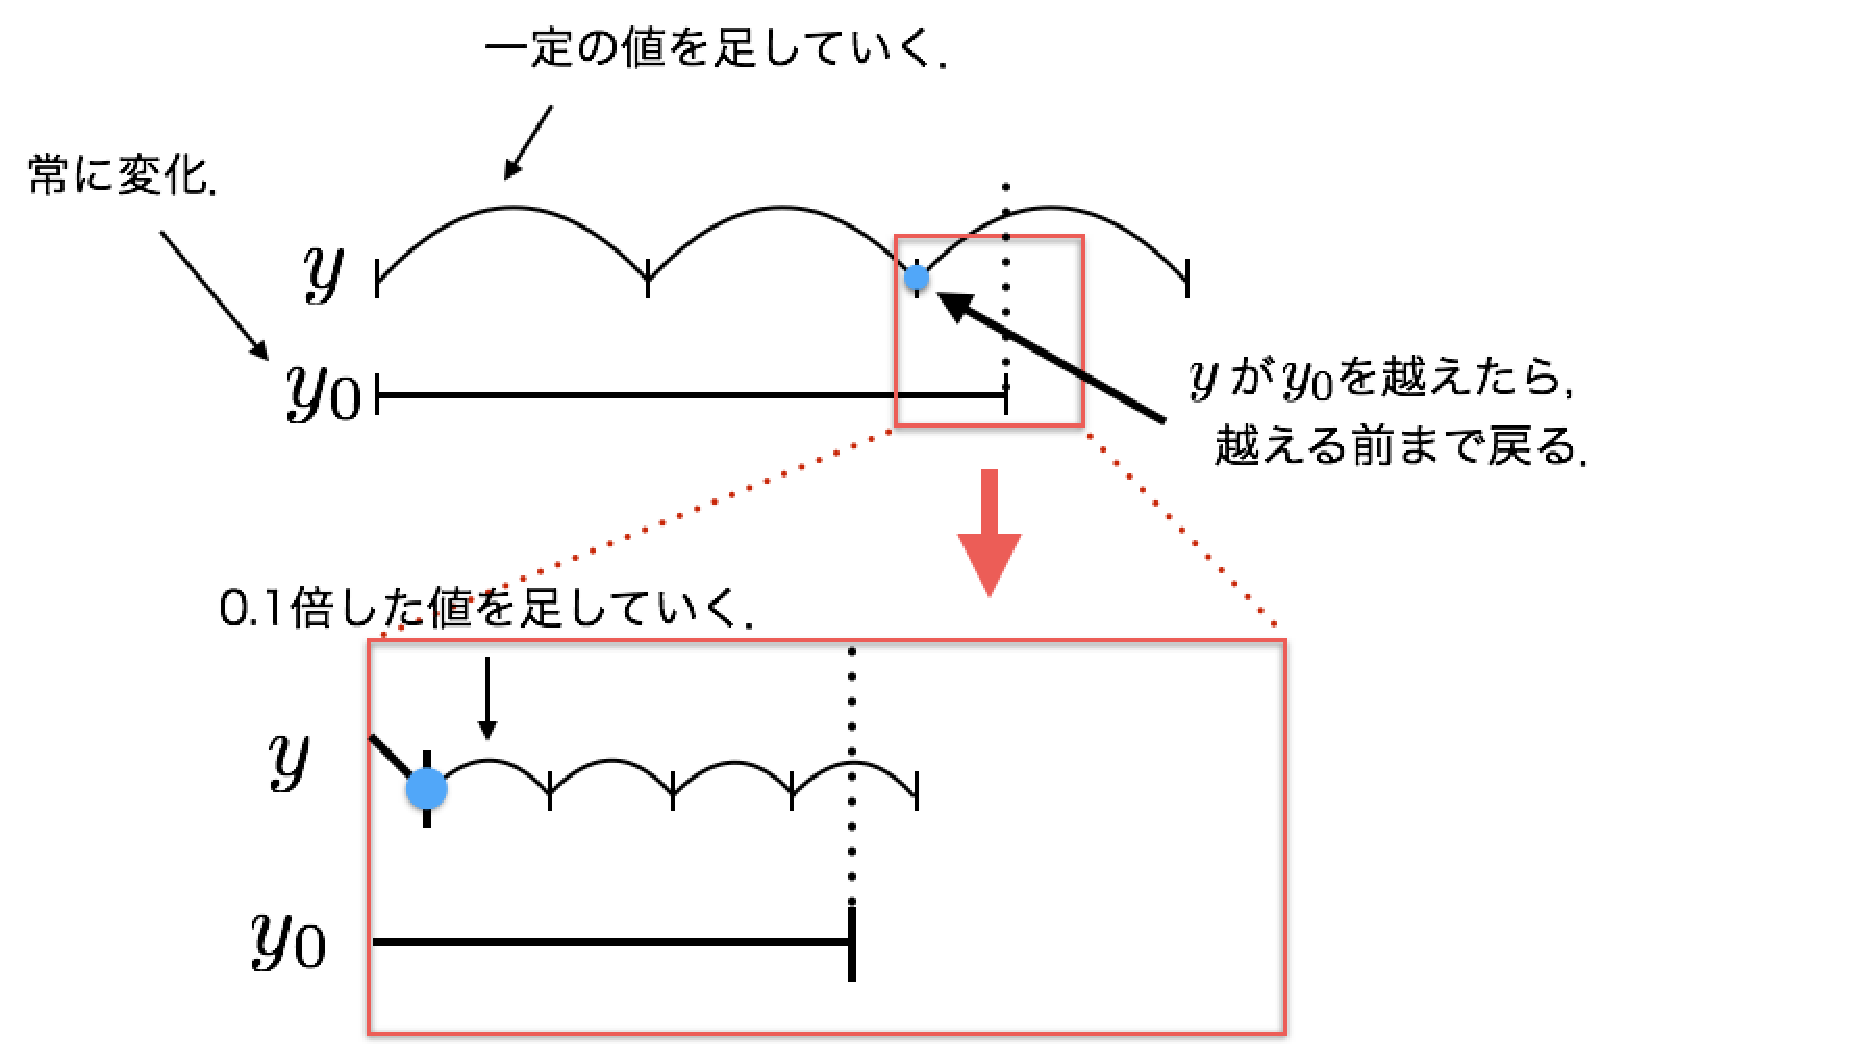
\includegraphics[width=130mm]{../image/fig2.eps}
 \end{center}
 \caption{熱膨張による変位決定アルゴリズム.}
 \label{fig:algo}
\end{figure}

\section{ペアポテンシャルによる計算}
\ref{sec:fcc}節でペアポテンシャルを利用したfcc構造での計算方法について記述した.
今回使用した経験的ペアポテンシャルは次式となる.
\begin{eqnarray}
\label{eq:method1}
U(r)=\frac{D}{n-m}\left[m{\left(\frac{r_0}{r}\right)}^n-n{\left(\frac{r_0}{r}\right)}^m\right]
\end{eqnarray}
このポテンシャルはLennart-Jones型であり,$r$が原子間距離,$r_0$が最安定距離,$D$,$n$,$m$は原子によって定まるパラメータである.また,$a_0$は計算に用いた平衡原子間距離である.
Cu, Ag, Auのパラメータを表\ref{tb:potential}に示す.例としてCuのポテンシャルの概形を図\ref{fig:lj}に示す.
\begin{table}[htbp]
\caption{ポテンシャルのパラメータ.}
  \label{tb:potential}
  \centering
  \begin{tabular}{cccccc}\hline
    元素 & $D$[J] & $n$ & $m$ & $r_0[\mathrm{\AA}$] & [$a_0\mathrm{\AA}$]\\ \hline \hline
    Cu & 2.8480708$\times10^{-20}$ & 9.0 & 5.5 & 2.5487 & 2.512666\\
    Ag & 2.295742359$\times10^{-20}$ & 11.5 & 5.50 & 2.876 & 2.846223\\
    Au & 3.23278851$\times10^{-20}$ & 10.5 & 5.50 & 2.8751 & 2.841578\\ \hline
  \end{tabular}
\end{table}
\begin{figure}[htbp]
 \begin{center}
  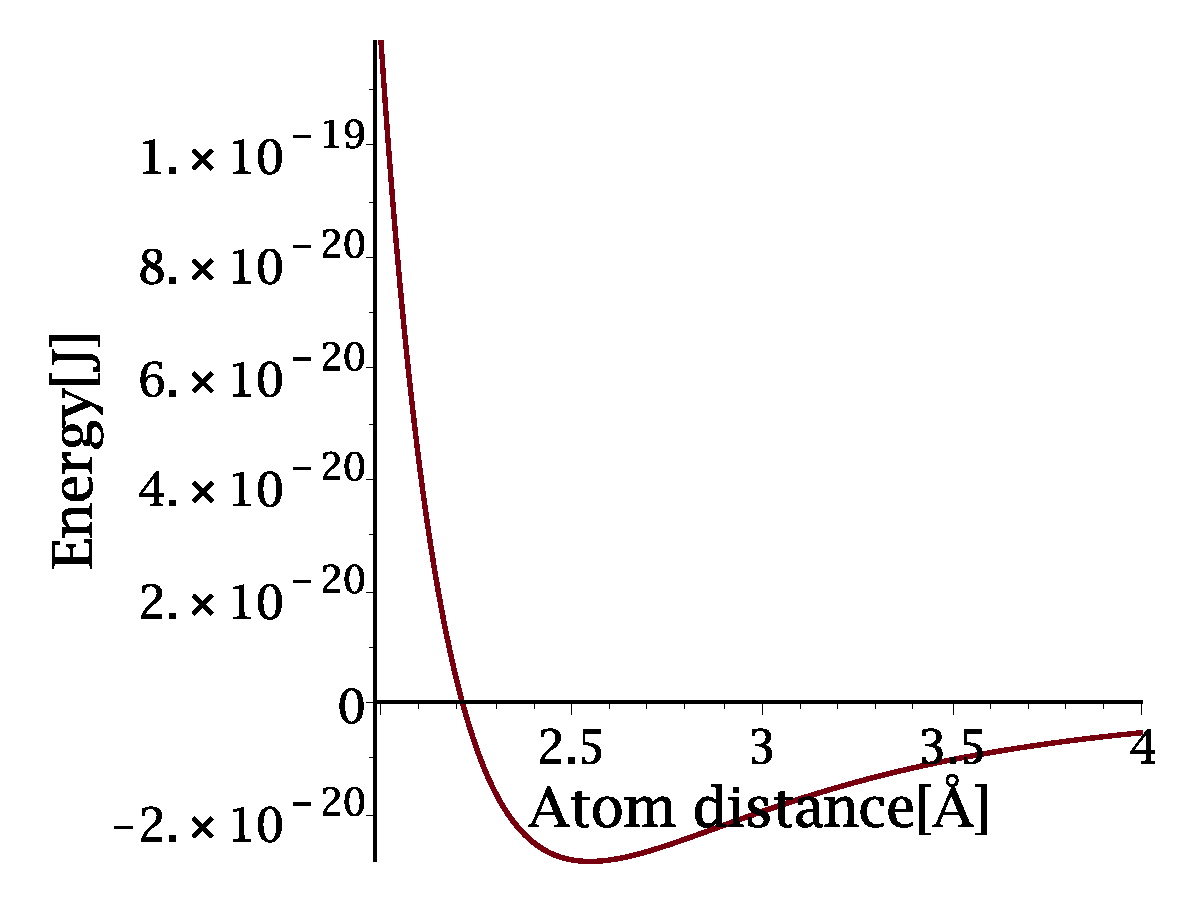
\includegraphics[width=100mm]{../image/lj.eps}
 \end{center}
 \caption{Cuのポテンシャルの概形.}
 \label{fig:lj}
\end{figure}
\section{VASPの導入}
Moment法はペアポテンシャルを前提としているが,VASPでの第一原理計算の結果の導入を試みる.
fcc構造であるCu, Ag, Au, Alのユニットセルの格子を変化させ,それぞれの基底状態のエネルギーを求める.
そして,フィッティングを行い最近接原子間距離とエネルギーについてのポテンシャル関数を作る.
このポテンシャル関数はVASPによる計算のため$x$,$y$,$z$全方位を考慮したポテンシャルである.
そのため,そのまま2次微分を$k$, 4次微分を6で割ったものを$\gamma$として式(\ref{eq:moment15})の$y_0$に入れて計算をしても$y_0$が線形結合を前提としているため上手く熱膨張を再現できない.
今回はfcc構造が当方的であることから,単純にポテンシャルを3で割り線形結合を表現することにする.
自由エネルギーの計算には式(\ref{eq:moment16})の線形結合の自由エネルギーに$k$, $\gamma$を代入し,式(\ref{eq:moment27})と同様に,$x, y, z$方向を考慮して3倍した値を自由エネルギーとする.
\subsection{VASP(Vienna Ab-initio Simulation Package)}
VASP は,密度汎関数法による平面波・擬ポテンシャル法を用いた第一原理計算プログラムパッケージで
ある.本研究ではこのソフトを用いて第一原理計算をおこなった.擬ポテンシャル法は原子の内殻電子を
除いた価電子だけを考慮する方法である.そのため,全電子を計算するフルポテンシャル法に比べ比較的
高速な計算が可能となる.また,内殻電子は化学結合や物性に影響を与えることが少ないのため,擬ポテ
ンシャル法であっても十分な精度で計算ができる.本研究の計算にはPAW法(Projector Augmented Wave method)を使用した.PAW法は擬ポテンシャル法を採用しながらも,内殻付近の挙動を比較的精度よく再現することができる計算手法である.VASPの計算条件は入力ファイルであるINCAR, KPOINTSにより決定される.本研究の中で比較をおこなった計算条件を以下に記す.
\begin{description}
 \item[ENCUT]\mbox{}\\ 
	    Cut-off energyと呼ばれる値である.
	    これは,どれだけ短波長の平面波を使い,波動関数をより精密に表現するかを決めるパラメータである.
	    入力した値が大きいほど,短波長の平面波を考慮に入れた計算を行うことができる.
 \item[KPOINTS]\mbox{}\\
	    波動関数を$k$空間で展開する際にどれだけの点をとるか決定することができる.
	    計算の精度に直接関わるパラメータである.
\end{description}


\subsection{フィッティング}
fcc構造のユニットセルに対して,VASPの構造最適化によって得られた格子定数を0.95倍から1.10倍まで0.01刻みで変化させエネルギーの計算を行い,得られた16点に対してフィッティングをおこなった.図\ref{fig:examplefit}にCuのフィッティングを示す.
\begin{figure}[htbp]
 \begin{center}
  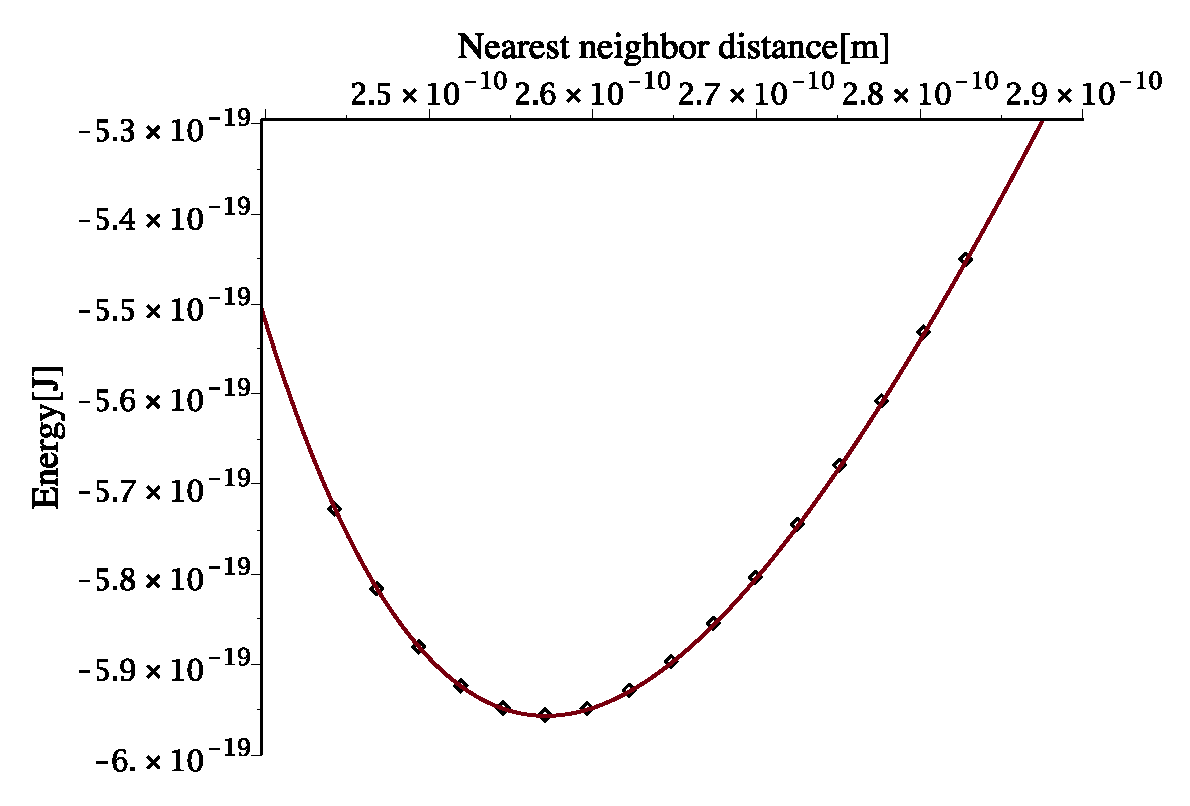
\includegraphics[width=100mm]{../image/fit5.eps}
 \end{center}
 \caption{Cuのフィッティング.}
 \label{fig:examplefit}
\end{figure}
今回フィッティングに使用した関数の$n$次数までの基本形は次式となる.
\begin{eqnarray}
\label{eq:method2}
U(r)=a_0+a_1(r-x_0)+a_2(r-x_0)^2+\cdots+a_n(r-x_0)^n
\end{eqnarray}
ここで,$x_0$はポテンシャルの最安定距離であり,関数全体を$x$方向に$x_0$だけずらしフィッティング精度を高めている.
フィッティングして得られたポテンシャルの2次,4次微分を利用することとなるが,4次微分となるとフィッティングの精度の影響を大きく受けてしまう.
また,フィッティング関数の次数もどこまで取れば最適なのか検討する必要がある.
図\ref{fig:fit}にフィッティングで得られた関数の4次微分の結果を示す.

\begin{figure}[htbp]
 \begin{minipage}[b]{0.5\linewidth}
  \centering
  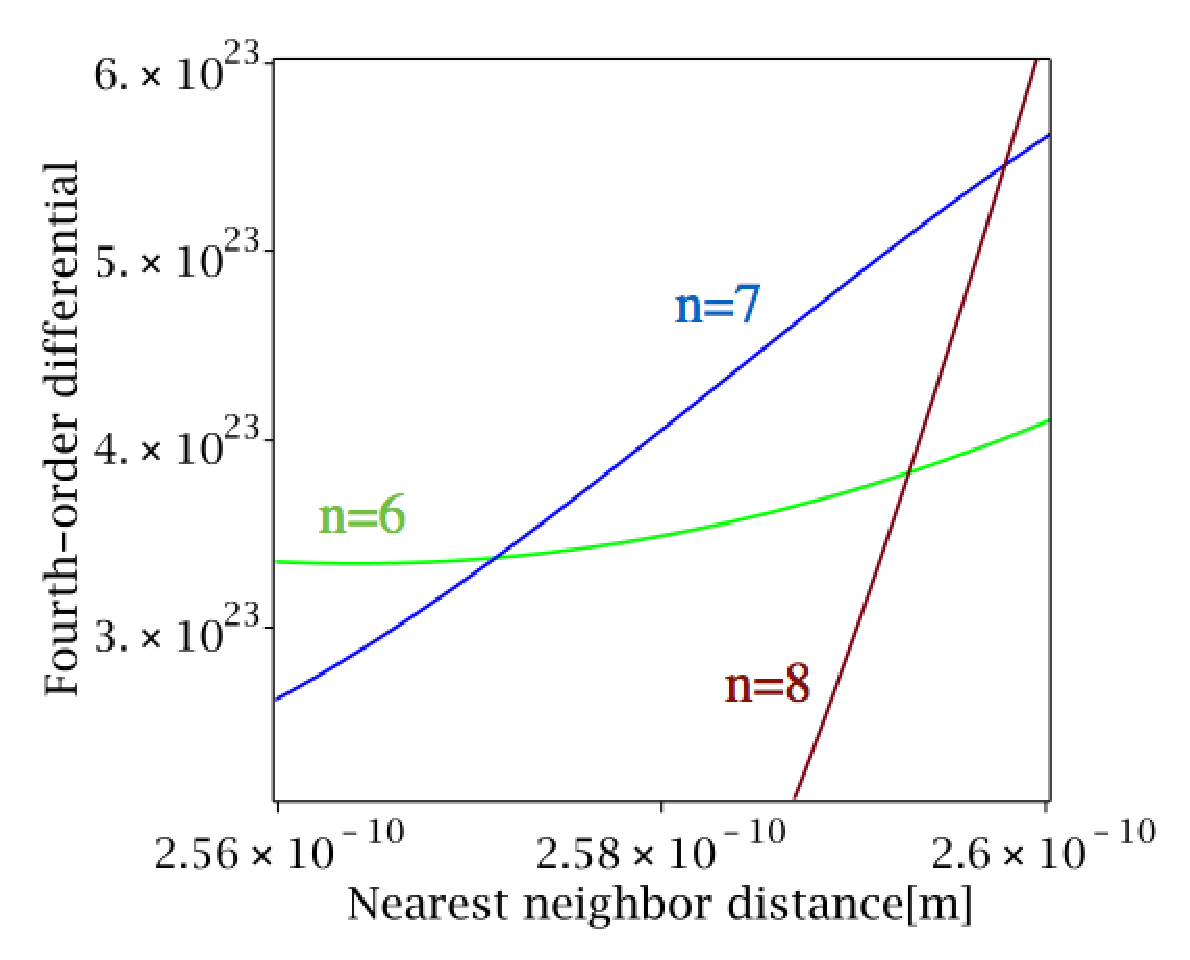
\includegraphics[keepaspectratio, scale=0.41]
  {../image/fit1label.eps}
  \subcaption{Cu, ENCUT=500, KPOINTS=6$\times$6$\times$6.}\label{fit1}
 \end{minipage}
 \begin{minipage}[b]{0.5\linewidth}
  \centering
  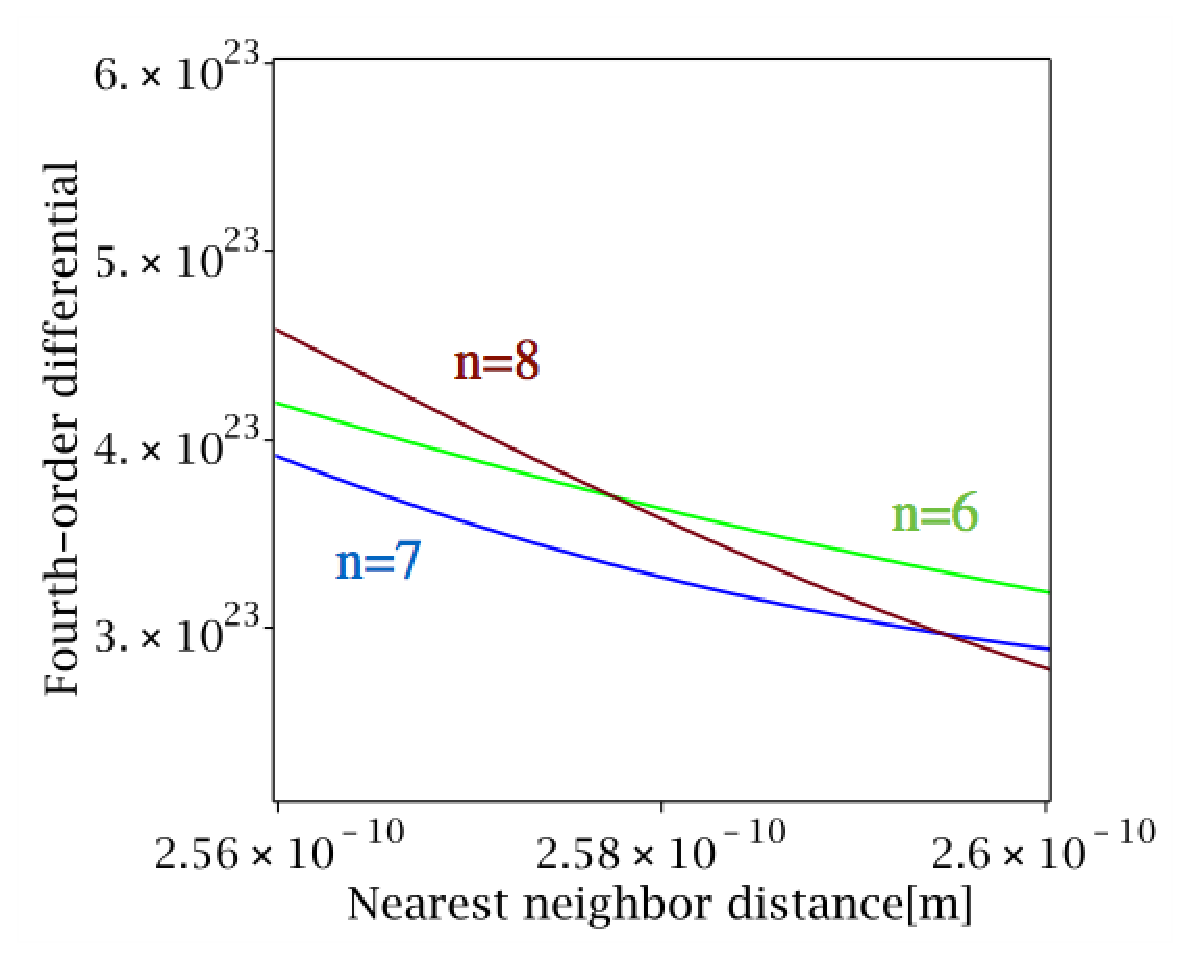
\includegraphics[keepaspectratio, scale=0.41]
  {../image/fit2label.eps}
  \subcaption{Cu, ENCUT=750, KPOINTS=12$\times$12$\times$12.}\label{fit2}
 \end{minipage}
 %\hspace{10cm}
 \begin{minipage}[b]{0.5\linewidth}
  \centering
  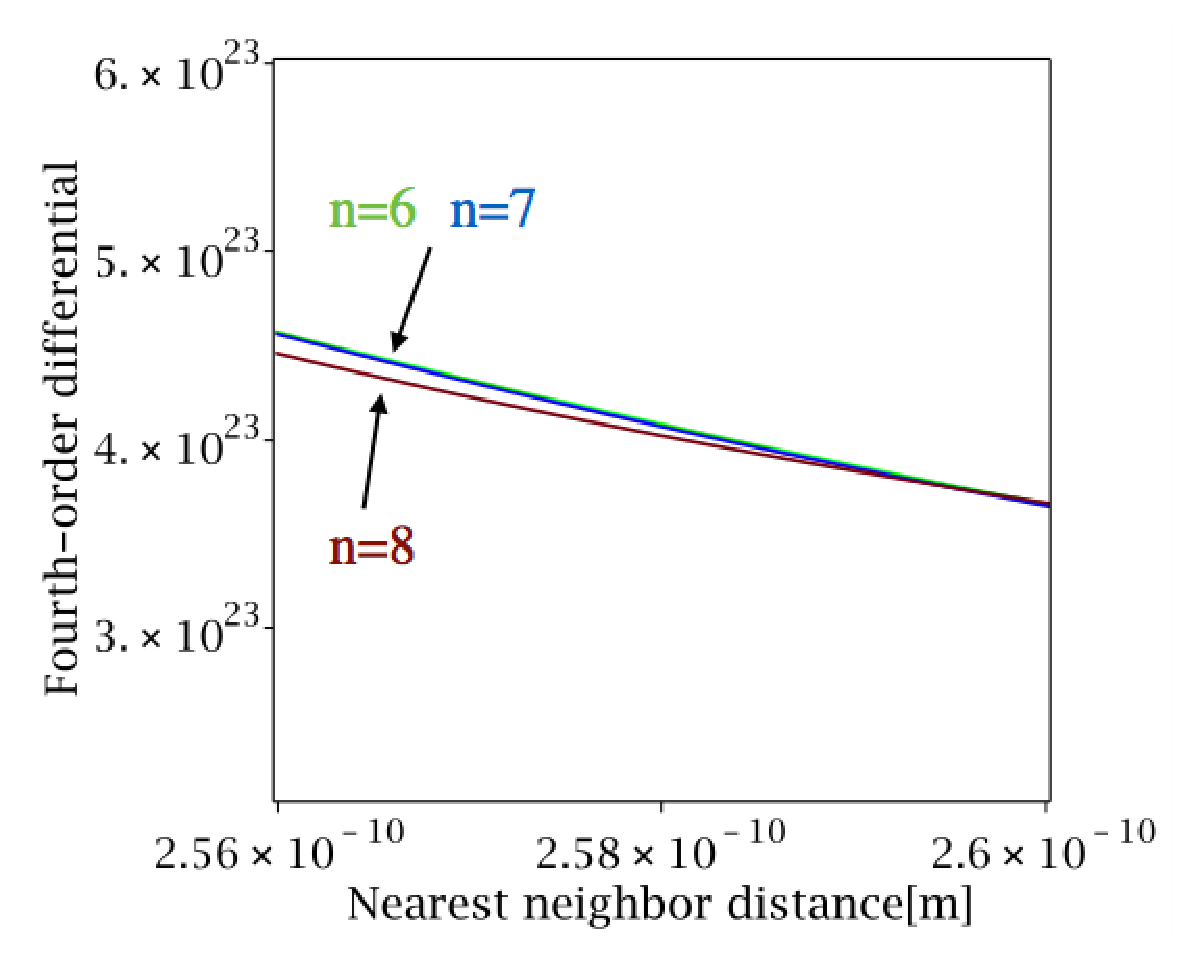
\includegraphics[keepaspectratio, scale=0.41]
  {../image/fit3label.eps}
  \subcaption{Cu, ENCUT=1000, KPOINTS=36$\times$36$\times$36.}\label{fit3}
 \end{minipage}
 \begin{minipage}[b]{0.5\linewidth}
  \centering
  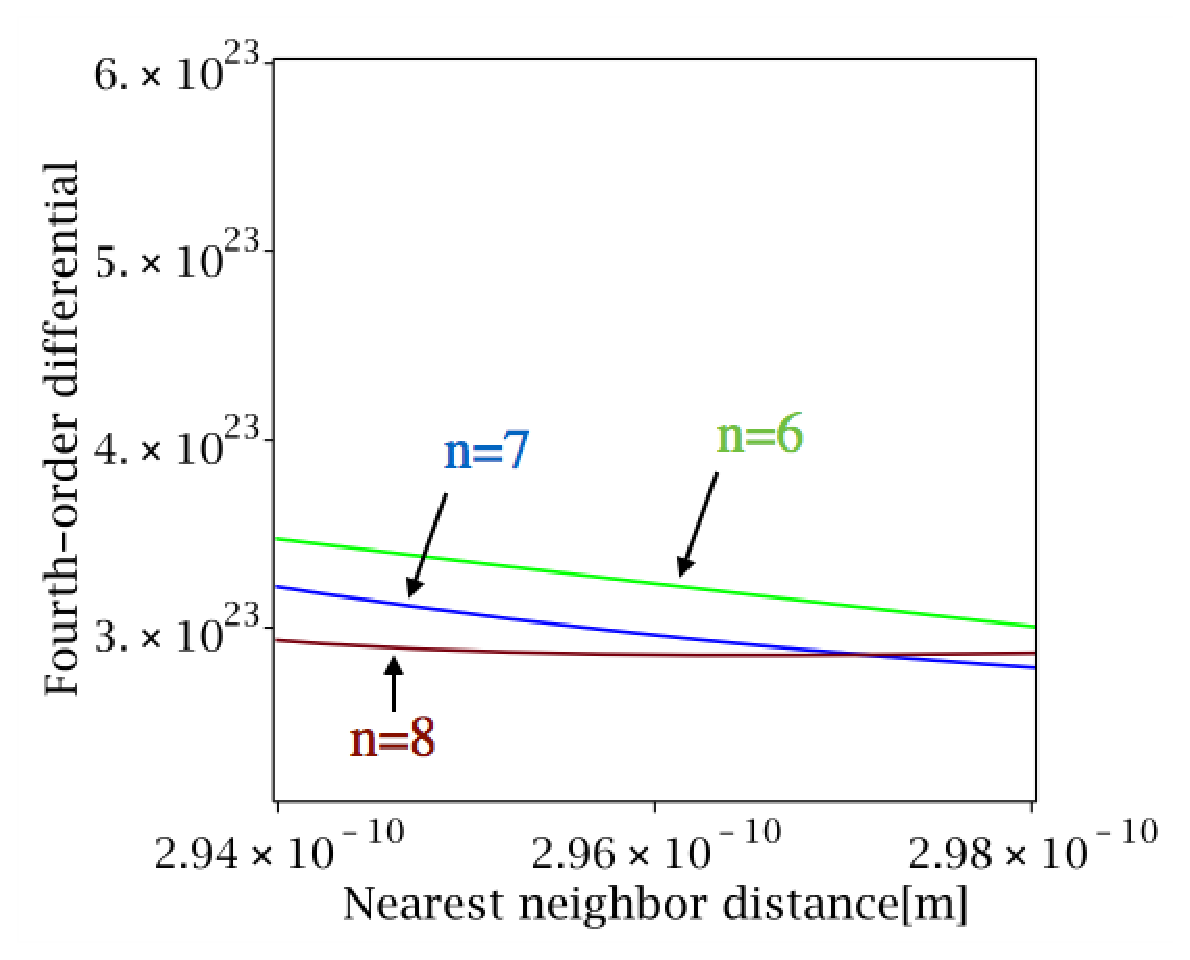
\includegraphics[keepaspectratio, scale=0.41]
  {../image/fit_ag_label.eps}
  \subcaption{Ag, ENCUT=1000, KPOINTS=36$\times$36$\times$36.}\label{fit4}
 \end{minipage}
  \begin{minipage}[b]{0.5\linewidth}
  \centering
  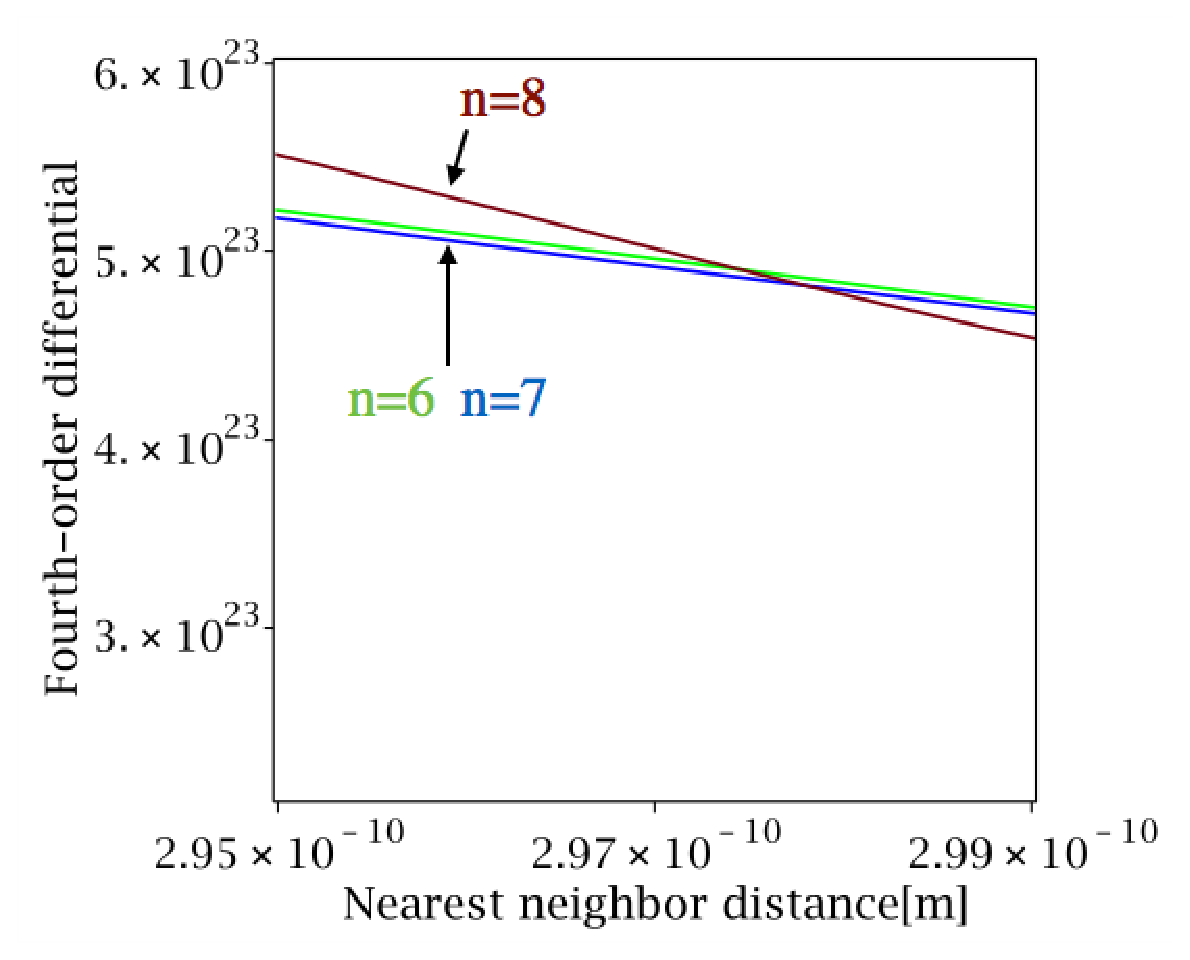
\includegraphics[keepaspectratio, scale=0.41]
  {../image/fit_au_label.eps}
  \subcaption{Au, ENCUT=1000, KPOINTS=36$\times$36$\times$36.}\label{fit5}
 \end{minipage}
 \begin{minipage}[b]{0.5\linewidth}
  \centering
  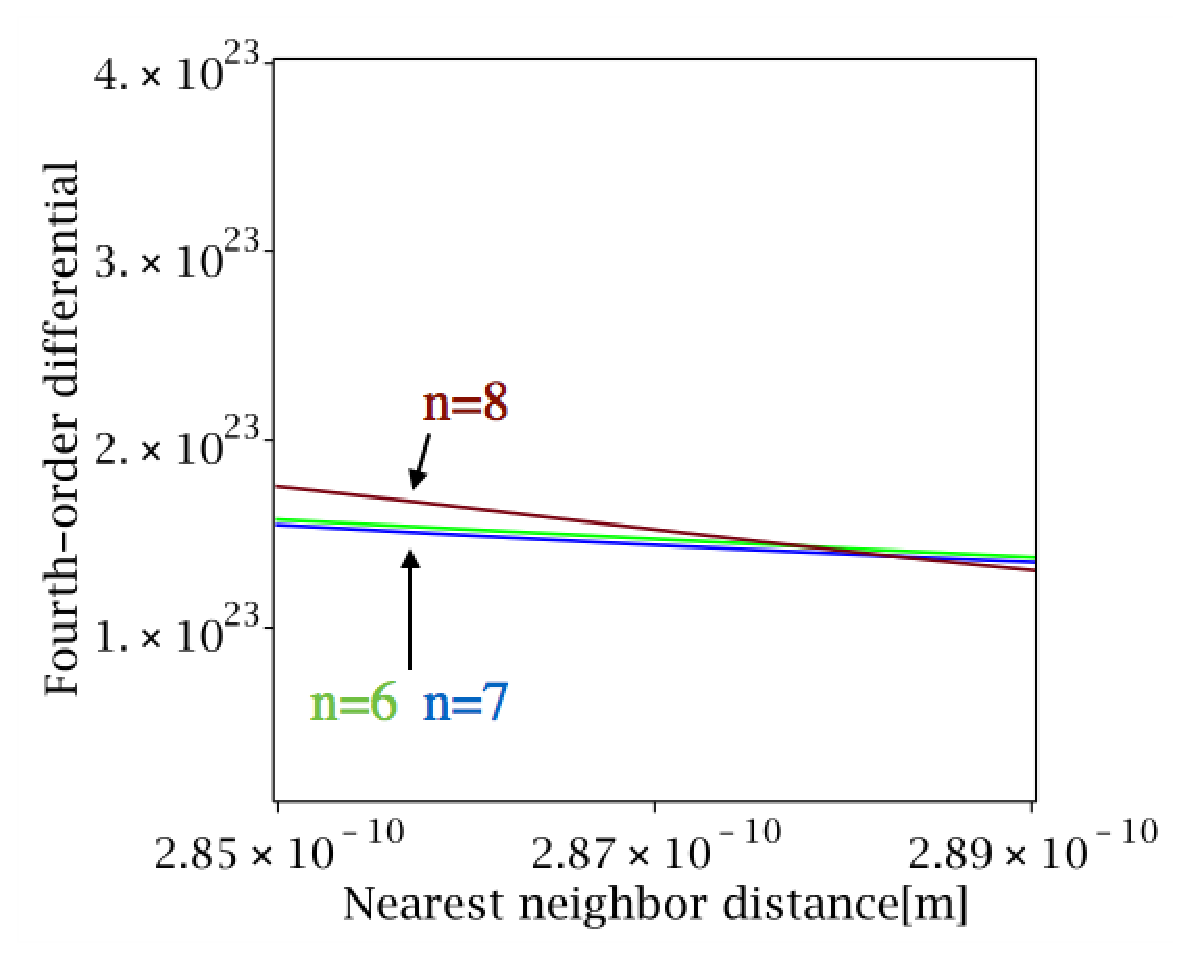
\includegraphics[keepaspectratio, scale=0.41]
  {../image/fit_al_label.eps}
  \subcaption{Al, ENCUT=1000, KPOINTS=36$\times$36$\times$36.}\label{fit6}
 \end{minipage}
 \caption{計算精度とフィッティング関数の次数によるポテンシャルの4次微分の値.$n$はフィッティングに使用した関数の次数である.ENCUT, KPOINTSはVASPの計算精度に関わるパラメータである.}\label{fig:fit}
\end{figure}

これは,フィッティング関数の次数とVASPの計算精度に関わるパラメータENCUTとKPOINTSによって,4次微分がどのような値をとるか示している.
横軸には各元素のVASPの構造最適化によって得られた最安定距離周辺を取っている.
図\ref{fig:fit}(\subref{fit1}),(\subref{fit2}),(\subref{fit3})はVASPの計算精度を変えることによって,Cuのフィッティング関数の4次微分にどのように変化するか示している.計算精度を高めることによって値が収束していることがわかる.
また,(\subref{fit4}),(\subref{fit5}),(\subref{fit6})は(\subref{fit3})と同じ計算条件のAg, Au, Alの結果である.
それぞれの結果を見るとAgを除けば6次と7次のフィッティング関数の値がほぼ一致するという結果であった.
8次のフィッティング関数に7次まででは拾えていない成分がある可能性もあるが,今回は4次微分した際に3次の項まで残れば十分であると判断し7次のフィッティング関数を用いてフィッティングを行う.
また,VASPでの計算条件はENCUT=1000,KPOINTS=36$\times$36$\times$36とする.
VASPの構造最適化で得られた実際の計算に用いた平衡原子間距離$a_0$を表\ref{tb:a0all}に示す.
7次のフィッティングで得られた2次微分,4次微分の値を図\ref{fig:allkgamma}に示す.
この図は,各元素の2次微分と4次微分のそれぞれ平衡原子間距離$a_0$からプロットし,値や傾きの比較が行えるようになっている.
\begin{table}[htbp]
\caption{VASPの構造最適化によって得られた平衡原子間距離$a_0$.}
  \label{tb:a0all}
  \centering
  \begin{tabular}{ccccc}\hline
    元素 & Cu & Ag & Au & Al\\ \hline \hline
    $a_0[\mathrm{\AA}]$ & 2.571623 & 2.944229 & 2.951082 & 2.856525\\ \hline
  \end{tabular}
\end{table}

\begin{figure}[htbp]
 \begin{minipage}[b]{0.5\linewidth}
  \centering
  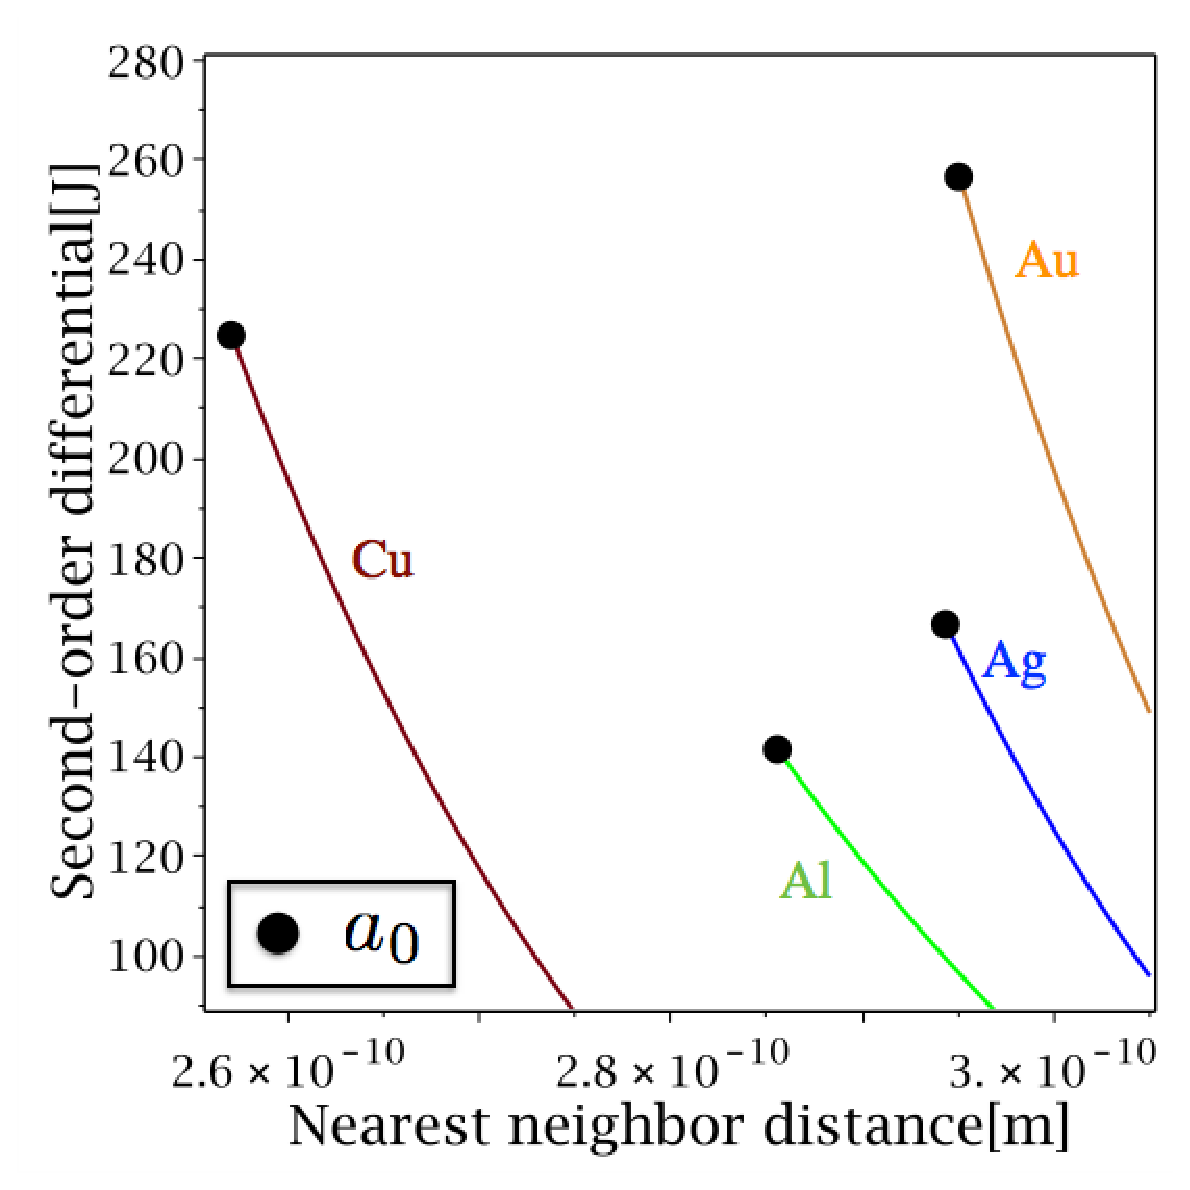
\includegraphics[keepaspectratio, scale=0.41]
  {../image/all_k_label.eps}
  \subcaption{フィッティングした関数の2次微分.}\label{allk}
 \end{minipage}
 \begin{minipage}[b]{0.5\linewidth}
  \centering
  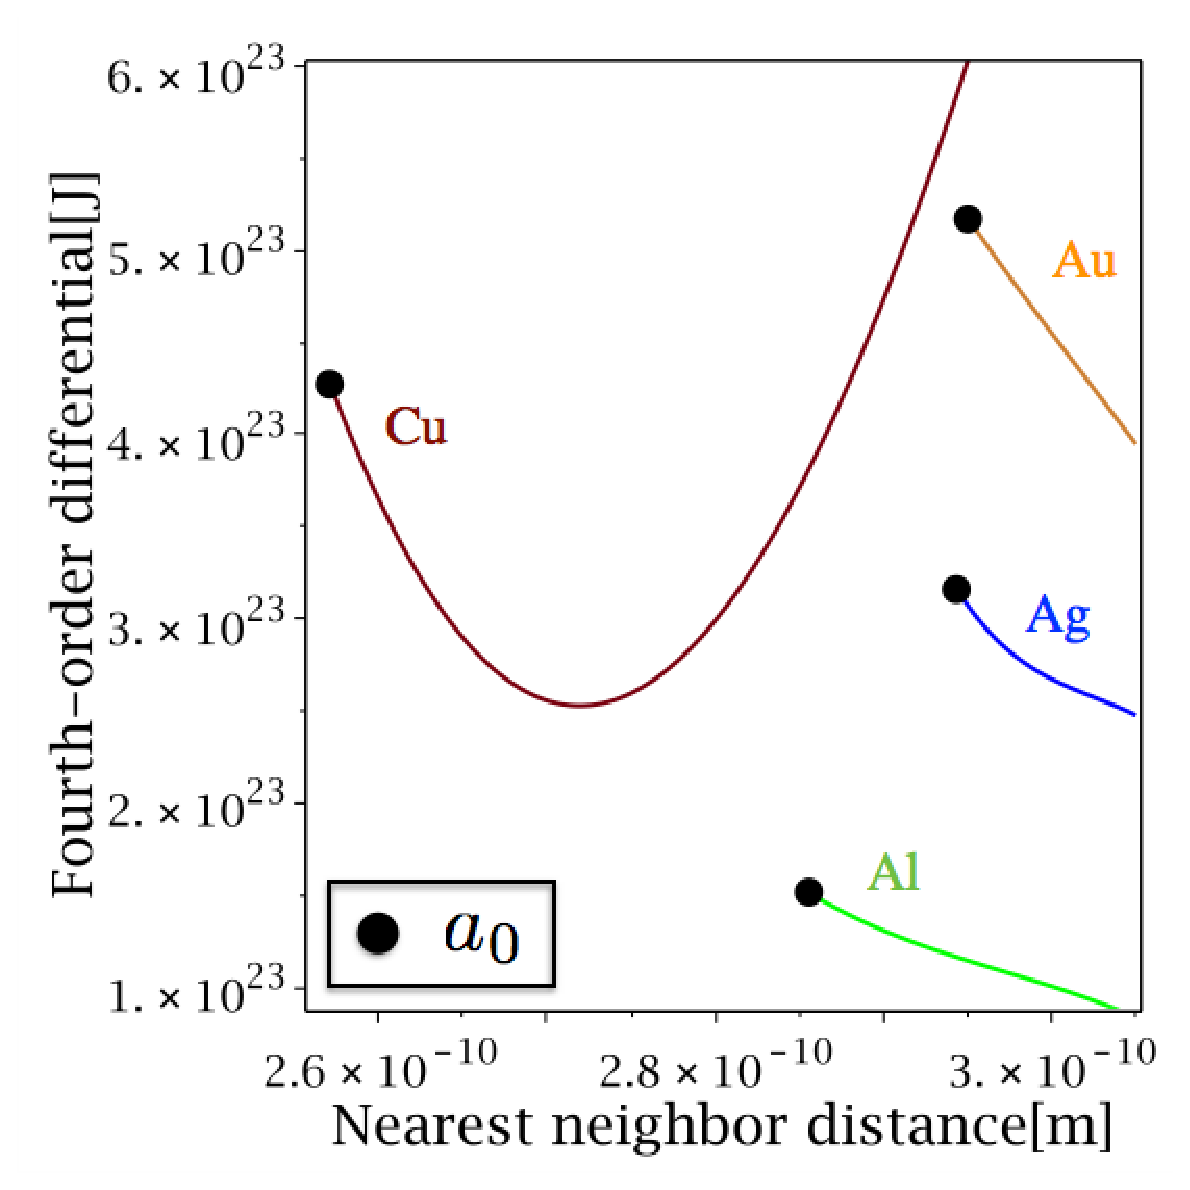
\includegraphics[keepaspectratio, scale=0.41]
  {../image/all_gamma_label.eps}
  \subcaption{フィッティングした関数の4次微分.}\label{allgamma}
 \end{minipage}
  \caption{各元素のフィッティングによって得られた関数の2次微分,4次微分の分布.}\label{fig:allkgamma}
\end{figure}


\section{MedeA}
データベースと第一原理計算を統合した材料設計支援のためのソフトウェアであり, 
構造の検索, 構築, 編集, 計算, 解析までを1つのプラットフォームで行うことができる商用ソフトである.
MedeAには格子振動に関連する物性を計算するためのツールとしてMedeA-Phononが搭載されており,擬調和振動子近似に基づき基底状態におけるPhonon分散曲線からPhonon状態密度を計算することができ,Phonon-DOS法を用いて自由エネルギーを算出することができる.
本研究ではMoment法の比較対象として,Cu,Ag,Au,Alの熱膨張と自由エネルギーの計算をおこなった.
Phonon-DOS法は熱振動効果を考慮しているが熱膨張は取り入れることができず,一定体積における自由エネルギーの計算を行うことになる.
そのため熱膨張を見積もるためには計算モデルの格子定数を変化させ,それぞれの自由エネルギーを算出し各温度における最安定構造を見つけ出す必要がある.
\subsection{Phonon-DOS法}
有限温度の効果を取り込んだ自由エネルギーは基底状態における系のトータルエネルギーと振動自由エネルギーの総和で表せられ次式で求めることができる\cite{kittel}.
\begin{eqnarray}
\label{eq:phonon}
F(a,T)=E(a)+k_BT\int_0^\infty n(\omega)\left[
2\sinh\left(\frac{\hbar\omega}{2k_BT}\right)
\right]d\omega
\end{eqnarray}
$E(a)$は基底状態の系のエネルギー,$k_B$はボルツマン定数,$T$は温度,$\omega$はPhonon分散曲線における振動数,$n(\omega)$はPhonon状態密度(Phonon-DOS),$\hbar$はプランク定数を$2\pi$で割った値である.
右辺第一項は基底状態におけるトータルエネルギー,右辺第二項は振動自由エネルギーを表している.
この式から振動自由エネルギーはPhonon状態密度から見積もることができ,Phonon状態密度を現実の系に近づけることが計算精度を高めることに繋がる.

\section{Phonopy}
東後篤史が制作したオープンソースのソフトウェアでありPhonon状態密度や分散曲線,自由エネルギーな
どの様々な有限温度の物性を第一原理計算ソフトと連携することで計算することができる\cite{phonopy}.
Phonopyという名前の由来は,Phonon計算をプラグラミング言語Pythonで行うことから来ている.
CLI(Command Line Interface)であり,Pythonのパッケージ管理システムであるpipとcondaに対応しており,環境構築も容易に行うことができる.
Phonon計算の簡単な流れは次のようになる.
\begin{enumerate}
 \item Phonopyにより原子を微小移動させたモデルを作成する.
 \item そのモデルに第一原理計算を行い,結果から力の定数を取り出す.
 \item 力の定数からPhonopyがPhonon計算を行う.
\end{enumerate}

Phonopyは内部エネルギー(基底状態のエネルギー)を考慮に入れた熱膨張を計算することが可能であり,それにより内部エネルギーと熱膨張を考慮に入れた自由エネルギーを見積もることができる.
本研究ではMoment法の比較対象として,Phonopyを用いて,Cu,Ag,Au,Alの熱膨張,自由エネルギー,内部エネルギーと熱膨張を考慮にいれた自由エネルギーの比較をおこなった.
\subsection{計算精度の検討}
PhonopyはVASPの計算から力の定数を取り出しPhononを計算するためVASPの計算結果に大きく依存する.
また,Phonon計算時に生じた誤差は温度の上昇とともに増大するため,高温域の状態を確認したいのであれば計算精度を高める必要がある.
計算精度による熱膨張の変化を図\ref{fig:phonopy}に示す.
図\ref{fig:phonopy}(\subref{phonopy1}),(\subref{phonopy2}),(\subref{phonopy3})はPhonopyによるAlの熱膨張の結果である.VASPの計算精度に関わるパラメータENCUTとKPOINTSを変えることによって,Phonopyの熱膨張の計算結果がどのように変わるか示している.
左側のグラフは横軸に体積,縦軸に自由エネルギーを取っており,各温度でフィッティングを行い最安定の体積を求めている.一番上のフィッティングカーブが0Kであり,一番下が1000Kと100K刻みで計算をしている.
中央のグラフは横軸に温度,縦軸に体積をとっており,左のグラフから得られる各温度での最安定の体積である..
右側のグラフは横軸に温度,縦軸に体積膨張係数を取っており,中央のグラフの温度微分である.
(\subref{phonopy1}),(\subref{phonopy2}),(\subref{phonopy3})を比較すると左側のグラフの高温域の点のずれが計算精度を高めることによって小さくなることがわかる.
このずれがフィッティングによる最安定点の決定に与える影響は大きく,体積膨張係数を見ればその影響力の大きさがよくわかる.
(\subref{phonopy3})の結果も,よく見ると点が線の中心からずれているため本来であればもっと計算精度を高めたいところである.
しかし,計算時間の都合もあり本研究のPhonopyの計算条件にはENCUT750,KPOINTS=12$\times$12$\times$12を使用した.


\begin{figure}[htbp]
 \begin{minipage}[b]{1.0\linewidth}
  \centering
  \includegraphics[keepaspectratio, scale=0.45]
  {../image/figure_1.png}
  \subcaption{ENCUT=500, KPOINTS=6$\times$6$\times$6.}\label{phonopy1}
 \end{minipage}
  \begin{minipage}[b]{1.0\linewidth}
  \centering
  \includegraphics[keepaspectratio, scale=0.45]
  {../image/figure_2.png}
  \subcaption{ENCUT=500, KPOINTS=12$\times$12$\times$12.}\label{phonopy2}
 \end{minipage}
   \begin{minipage}[b]{1.0\linewidth}
  \centering
  \includegraphics[keepaspectratio, scale=0.45]
  {../image/figure_3.png}
  \subcaption{ENCUT=750, KPOINTS=12$\times$12$\times$12.}\label{phonopy3}
 \end{minipage}
 \caption{VASPの計算精度によるPhonopyのAlの熱膨張の計算誤差.}\label{fig:phonopy}
\end{figure}



